% Required packages: graphicx, amsmath, booktabs, and xcolor with the table option.
\subsection{Provider Assurance Overhead}
\label{sec:evaluation-assurance}

We evaluate scoped proof-based assurance and the isolated signing component
of the TEE-based path. Proof measurements replay retained witnesses from
128 Qwen3-1.7B requests comprising 1,024 calls on the B300 server CPU;
model inference is excluded. The circuit enforces the scoped accounting
commitment, integer token charges, and scoped request-hash equality, while
receipt-bound witness validation and shared-field linkage checks execute
on the host. Values are means and sample standard deviations across three
rounds or paired signing sessions. Appendix~\ref{app:c-assurance} provides
the measurement boundaries and complete results.

\noindent\textbf{Scoped proof costs.}
Table~\ref{tab:c-assurance-components} summarizes the component costs.
With persistent CPU workers, circuit witness calculation and proving take
148.45 $\pm$ 7.64\,ms/call, and verification takes
15.10 $\pm$ 1.55\,ms/call. The serialized JSON proof occupies
722.98 $\pm$ 0.47\,B/call. These measurements quantify the scoped
assurance operation used by the prototype. The original process-per-call
adapter and the persistent implementation are reported separately in
Table~\ref{tab:c1-assurance-cost}.

\begin{table}[!t]
\centering
\caption{Assurance component costs (mean $\pm$ sample SD across three proof rounds or signing sessions).}
\label{tab:c-assurance-components}
\footnotesize
\renewcommand{\arraystretch}{1.08}
\begin{tabular*}{\columnwidth}{@{\hspace{3pt}}l@{\extracolsep{\fill}}cc@{\hspace{3pt}}}
\toprule
\textbf{Component} & \textbf{Unit} & \textbf{Mean $\pm$ SD} \\
\midrule
\rowcolor{gray!12}
\multicolumn{3}{@{\hspace{3pt}}l@{\hspace{3pt}}}{\textbf{Scoped Groth16 (B300 server CPU)}} \\
Circuit witness + proving & ms/call & 148.45 $\pm$ 7.64 \\
Proof verification & ms/call & 15.10 $\pm$ 1.55 \\
Serialized proof (JSON) & B/call & 722.98 $\pm$ 0.47 \\
\midrule
\rowcolor{gray!12}
\multicolumn{3}{@{\hspace{3pt}}l@{\hspace{3pt}}}{\textbf{TEE-based receipt signing (local)}} \\
Software-key signing & ms/receipt & 0.534 $\pm$ 0.028 \\
TEE-based signing & ms/receipt & 0.763 $\pm$ 0.085 \\
\textbf{Paired signing increment} & ms/receipt & \textcolor[HTML]{2E3B97}{\textbf{0.229 $\pm$ 0.108}} \\
\bottomrule
\end{tabular*}
\end{table}

\noindent\textbf{Immediate versus deferred proving.}
Figure~\ref{fig:c-deferred-audit}(a) varies the number of calls per request
from one to eight. Immediate generates proofs in the foreground and verifies
them during the subsequent audit; Deferred performs both operations during
audit. Both modes revalidate and prepare witnesses and persist a fresh copy
before the foreground phase ends. At eight calls, Deferred reduces foreground
protocol time from 1,200.07 $\pm$ 60.99 to
8.65 $\pm$ 2.48\,ms/request, a within-round reduction of
99.28\% $\pm$ 0.19 percentage points.
The subsequent Deferred audit takes 1,332.92 $\pm$ 39.68\,ms/request.
Total replay processing is 1,317.54 $\pm$ 74.00\,ms/request for Immediate
and 1,341.56 $\pm$ 42.14\,ms/request for Deferred: deferral moves proof work
off the foreground path while retaining its eventual processing cost.
These phase timings measure protocol replay, excluding LLM inference.

\begin{figure}[!t]
  \centering
  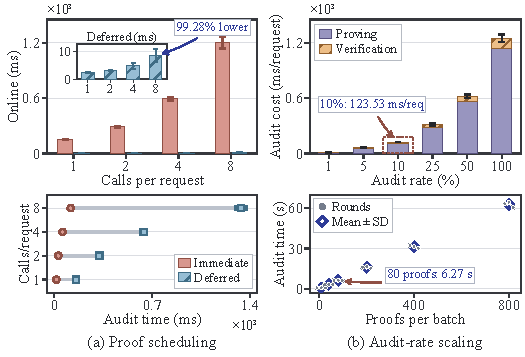
\includegraphics[width=\columnwidth]{c_deferred_proving_audit_rate.pdf}
  \caption{Proof scheduling and audit-rate scaling on retained serving
  witnesses. (a) Foreground protocol cost (upper) and subsequent audit time
  (lower); the inset enlarges Deferred foreground cost. The shared mode
  legend applies to both plots. (b) Proving and verification costs amortized
  over all 100 batch requests (upper), and elapsed audit time with two
  workers (lower), using eight calls per request. Error bars show sample SD
  across three rounds. Gray dots show round-level audit times with small
  horizontal offsets for visibility.}
  \label{fig:c-deferred-audit}
\end{figure}

\noindent\textbf{Audit-rate scaling.}
Figure~\ref{fig:c-deferred-audit}(b) varies the audited fraction from
1\% to 100\%. Each batch contains 100 requests, and auditing a request
checks all eight calls. Combined proving and verification cost increases
from 12.57 $\pm$ 0.47 to 1,248.94 $\pm$ 41.00\,ms/request
as the number of proofs grows from eight to 800.
At the default 10\% audit rate, 80 proofs incur an amortized cost of
123.53 $\pm$ 1.42\,ms/request, and two CPU workers complete the audit
batch in 6.27 $\pm$ 0.08\,s. The upper plot sums individual operation
wall times and divides by all batch requests; the lower plot measures actual
elapsed completion time. Proof generation remains in the audit phase at
every rate. Table~\ref{tab:c3-audit-rate} reports the complete scan.

\noindent\textbf{TEE-based receipt signing.}
We separately compare local TEE-based isolated-key signing with a
software-key control using the same ECDSA-P256 API. Each mode signs
1,024 retained receipts in each of three paired sessions.
TEE-based signing takes 0.763 $\pm$ 0.085\,ms/receipt, versus
0.534 $\pm$ 0.028\,ms/receipt for the software-key control.
The paired increment is 0.229 $\pm$ 0.108\,ms/receipt.
This experiment measures protected private-key operations;
receipt preparation and accounting remain on the host.
The 6,144 measured signatures verify successfully.
Table~\ref{tab:c4-tee-signing} includes hashing, verification, and session
key setup. Full inference attestation and remote attestation are outside
this component measurement.
